\section{Empirical results}\label{sec:results}
\subsection{Does the disappearing index effect appear in Sweden?}

The Swedish data show lower full-window returns than in the earliest period, but not a steady disappearance. Table~\ref{tab:returns} reports the announcement, implementation and full-window means. Addition CARs are 8.52\%, 0.25\%, 2.85\% and 1.50\% across the four successive periods. The large early value is followed by a near-zero mean and then a recovery. Figure~\ref{fig:period_returns} displays the estimates with their uncertainty, making that non-monotonic pattern explicit.

\begin{table}[!htbp]
\centering
\caption{Market adjusted returns around index changes}\label{tab:returns}
\small
\setlength{\tabcolsep}{5pt}
\begin{tabular}{llrrrrrlr}
\toprule
Type & Period & $N$ & $G$ & AD & ED & Total & 95\% interval & $p$ \\
\midrule
Addition & 2007--2011 & 33 & 9 & 0.96 & 1.16 & 8.52 & [2.46, 14.74] & 0.027 \\
Addition & 2012--2016 & 54 & 10 & 1.87 & -0.73 & 0.25 & [-3.73, 5.30] & 0.908 \\
Addition & 2017--2021 & 82 & 10 & -0.16 & 0.38 & 2.85 & [1.26, 5.20] & 0.005 \\
Addition & 2022--2026 & 87 & 9 & 1.20 & -0.09 & 1.50 & [-0.10, 3.22] & 0.062 \\
Deletion & 2007--2011 & 33 & 9 & -0.77 & -0.09 & -6.16 & [-11.41, -2.10] & 0.007 \\
Deletion & 2012--2016 & 46 & 10 & -1.71 & -0.85 & -2.47 & [-14.42, 3.60] & 0.522 \\
Deletion & 2017--2021 & 61 & 10 & -2.09 & 0.89 & -0.43 & [-3.43, 3.02] & 0.759 \\
Deletion & 2022--2026 & 75 & 9 & -0.71 & -1.23 & -1.53 & [-4.24, 0.89] & 0.279 \\
\bottomrule
\end{tabular}
\begin{minipage}{\linewidth}\footnotesize\vspace{5pt}
Returns are percentages. AD denotes CAR $[AD-1,AD+1]$, ED denotes CAR $[ED-1,ED+1]$, and Total denotes CAR $[AD-1,ED+1]$, where AD is the recorded announcement trading date and ED the effective trading date. The benchmark is OMXSBGI. Means weight events equally. $N$ and $G$ are event and review counts for Total; AD and ED use their own complete cases. Intervals and two-sided $p$-values for Total use the inherited restricted wild cluster bootstrap with 9,999 draws, Webb weights below 12 clusters and Rademacher weights otherwise. These are pointwise, exploratory intervals. No stars are used. Source: effect/tabell1\_lang.csv, panel A/B.
\end{minipage}
\end{table}


\begin{figure}[!htbp]\centering
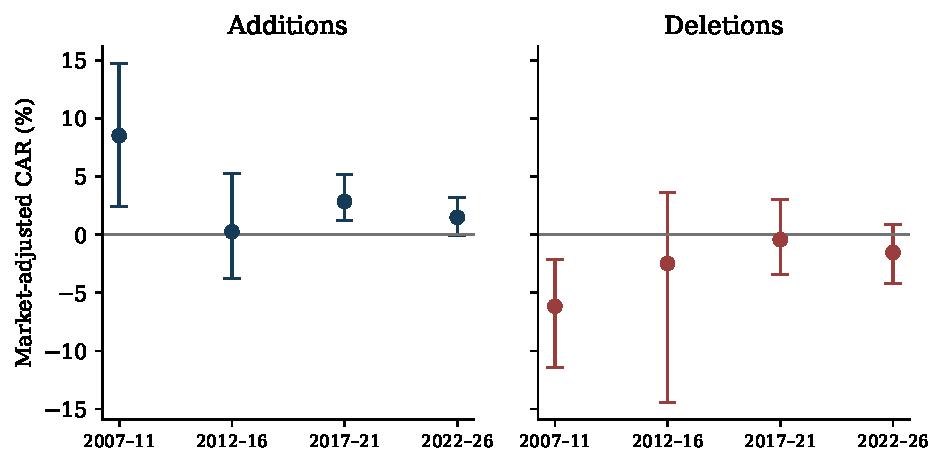
\includegraphics[width=.96\linewidth]{figures/period_returns.pdf}
\caption{Returns around OMXSB changes by period. Points are event-weighted mean CARs from AD-1 through ED+1; bars are the 95\% review-cluster wild-bootstrap intervals reported in Table~\ref{tab:returns}. The vertical scale is identical for additions and deletions. Periods begin in July 2007 and end in June 2026. The estimates describe observed index events, not a fitted trend.}\label{fig:period_returns}
\end{figure}

Deletions have negative means in all four periods: -6.16\%, -2.47\%, -0.43\% and -1.53\%. Their intervals are generally wider than those for additions. In particular, the 2012--2016 deletion estimate is sensitive to the weighting of large reviews. The sign of the averages is consistent with the conventional index-event pattern, but the sample does not precisely resolve the magnitude of recent deletion returns.

The published US finding in \citet{greenwood2025} is a useful benchmark for the question, not a directly comparable control group. Their published abstract reports an average S\&P 500 addition return below 1\% and deletion return of 0.1\% in 2010--2020. Sweden's later interval begins in 2017 and ends in 2026, uses a different benchmark and review institution, and contains different firms. We consequently ask whether a similarly small return is evident within the Swedish series, rather than subtracting the US number and calling the difference a country effect.

For 2017--2026 as a whole, addition CAR averages 2.15\%, with a 95\% interval of [1.01\%, 3.39\%], across 169 events and 19 reviews. The corresponding deletion mean is -1.04\%, with an interval of [-2.88\%, 0.90\%]. These are economically different levels of precision. 

The latest addition estimate, 1.50\%, has an interval of [-0.10\%, 3.22\%]. This permits both a near-zero average and a positive return of economically meaningful size. It does not establish disappearance. The latest block contains only nine review clusters, and its mean is sensitive to particular observations and overlapping index events, as shown below.

The direct time contrasts sharpen the answer. Latest minus earliest addition CAR is -7.03 percentage points, whereas latest minus preceding is -1.35 points, later minus earlier decade is -1.24 points, and the annual linear trend is -0.28 points. Only the endpoint contrast has a pointwise bootstrap interval excluding zero; that result does not survive the limited ten-test multiplicity adjustment. Table~\ref{tab:contrasts} in the appendix reports all contrasts. The evidence is therefore strongest for a high earliest-period mean and a positive later-decade association, rather than a statistically established smooth decline.

\subsection{How much does the changing event calendar matter?}

The full-window comparison covers the entire interval between announcement and implementation. In Sweden, that interval changes substantially. Among reviews represented in the complete addition sample, its median is 14, 16, 15 and 6 trading days in the four blocks. Thus, the latest full window is considerably shorter than the typical earlier window. This is a feature of the institution and measurement, not evidence by itself that timing caused any return difference.

We therefore calculate a fixed initial seven-day window, AD-1 through AD+5, on the same events as the full-window means. It contains seven daily returns and ends before implementation for every event. This choice was made after inspecting the event calendar, and the exercise is exploratory. Table~\ref{tab:timing} reports both windows and the remaining portion of the full window.

\begin{table}[!htbp]
\centering
\caption{The full event window and a common initial seven-day window}\label{tab:timing}
\small
\setlength{\tabcolsep}{5pt}
\begin{tabular}{llrrrrr}
\toprule
Type & Period & Events & Gap & Full & Initial seven & Remainder \\
\midrule
Addition & 2007--2011 & 33 & 14 & 8.52 & 1.19 & 7.34 \\
Addition & 2012--2016 & 54 & 16 & 0.25 & 1.26 & -1.01 \\
Addition & 2017--2021 & 82 & 15 & 2.85 & 1.23 & 1.62 \\
Addition & 2022--2026 & 87 & 6 & 1.50 & 1.80 & -0.31 \\
Deletion & 2007--2011 & 33 & 15 & -6.16 & -3.54 & -2.62 \\
Deletion & 2012--2016 & 46 & 16 & -2.47 & -0.86 & -1.61 \\
Deletion & 2017--2021 & 61 & 15 & -0.43 & -1.82 & 1.39 \\
Deletion & 2022--2026 & 75 & 6 & -1.53 & -0.76 & -0.77 \\
\bottomrule
\end{tabular}
\begin{minipage}{\linewidth}\footnotesize\vspace{5pt}
Returns are percentages. Gap is the median AD-to-ED distance in trading days across distinct reviews represented in the sample. Full includes AD-1 through ED+1; Initial seven includes AD-1 through AD+5; Remainder includes AD+6 through ED+1. Every row uses identical events and the two components sum to Full. The remainder has varying duration. This timing diagnostic is exploratory; uncertainty for period contrasts is reported in Appendix~\ref{app:inference}.
\end{minipage}
\end{table}


The addition initial seven-day means are 1.19\%, 1.26\%, 1.23\% and 1.80\%. The very high 8.52\% earliest full-window mean is therefore not a comparably high initial seven-day response: approximately 7.34 percentage points accrue in the remaining interval. In the latest block, the remainder is approximately -0.31 points. These are within-sample accounting comparisons; they do not establish that the initial seven-day population means are equal or that shortening the calendar explains the difference causally.

The distinction matters for the replication's economic interpretation. A declining full-event CAR need not be a declining immediate response to the announcement. It may reflect where returns occur along an episode whose duration also changes. Both parts of the evidence should be visible. The full window remains appropriate for the entire index change, while the fixed window prevents the early large CAR from being described as a large announcement-week reaction without checking its timing.

Return aggregation is a separate issue. On the same 169 later additions, replacing the arithmetic daily sum with compounded stock return minus compounded benchmark return changes the mean from 2.15\% to 2.18\%. In the latest block it changes 1.50\% to 1.45\%. The positive pooled later association is not created by this particular aggregation choice. Alternative closing-price endpoints are also shown in Appendix~\ref{app:data}; the daily return inclusion convention is kept explicit rather than treated as interchangeable with the window label.

\subsection{Composition, coincident index changes and anticipation}

Following the anchor study, we next ask whether changing observable characteristics account for the time pattern. Table~\ref{tab:composition} compares unadjusted and adjusted period estimates on identical complete-case samples. For latest-period additions, the estimate is 1.59\% without controls and 1.60\% with them. For early additions, the corresponding values are 8.97\% and 10.12\%. These controls do not explain away the difference in this specification.

\begin{table}[!htbp]
\centering
\caption{Composition adjustment on a common event sample}\label{tab:composition}
\small
\setlength{\tabcolsep}{5pt}
\begin{tabular}{llrrl}
\toprule
Type & Period & Unadjusted & Adjusted & Adjusted CR1 interval \\
\midrule
Addition & 2007--11 & 8.97 & 10.12 & [5.09, 15.16] \\
Addition & 2012--16 & 0.74 & 0.55 & [-3.01, 4.11] \\
Addition & 2017--21 & 2.64 & 2.33 & [0.38, 4.29] \\
Addition & 2022--26 & 1.59 & 1.60 & [0.68, 2.53] \\
Deletion & 2007--11 & -5.66 & -6.23 & [-11.03, -1.43] \\
Deletion & 2012--16 & -1.37 & -1.42 & [-7.61, 4.76] \\
Deletion & 2017--21 & -0.77 & -0.29 & [-3.35, 2.77] \\
Deletion & 2022--26 & -1.83 & -1.95 & [-4.02, 0.12] \\
\bottomrule
\end{tabular}
\begin{minipage}{\linewidth}\footnotesize\vspace{5pt}
Period intercepts from CAR $[AD-1,ED+1]$ regressions. Both columns use the same complete-case sample: 237 additions or 185 deletions. Adjusted estimates control for centered abnormal turnover, relative size, residual return variance and analyst coverage. The columns are not a causal decomposition. Intervals are analytical CR1 review-clustered intervals using $t_{G-1}$; unstable inverted bootstrap intervals from auxiliary sparse specifications are not used here. Source: composition/tabell2\_tabell4.csv, table 2.
\end{minipage}
\end{table}


The comparison is conditional on the available turnover, size, residual-variance and analyst-coverage proxies. It does not prove that composition is irrelevant. Missing controls reduce the sample to 237 additions and 185 deletions, and the proxies do not capture all reasons for membership changes. The common-sample unadjusted column is important: comparing an adjusted result with a larger raw sample would otherwise attribute selection from missing controls to the controls themselves.

Coincident MSCI changes matter for magnitudes. Excluding them lowers the later addition mean from 2.15\% to 1.46\%, with an interval of [0.50\%, 2.47\%]. The latest mean falls from 1.50\% to 0.73\%, with an interval including zero. Overlapping events have unusually large returns. This is a Swedish counterpart to asking whether index-specific institutional details change measured demand, but it is not the US migration mechanism: removing an overlap does not identify the incremental causal contribution of either index.

Table~\ref{tab:robustness} also excludes Sivers separately, applies winsorization, and removes observations flagged in a targeted company-news review. The later-decade addition mean remains positive with an interval excluding zero in these individual checks. The latest-block mean is more sensitive. The news screen covers the 24 most extreme events, so its remaining observations cannot be described as comprehensively news-free.

\begin{table}[!htbp]
\centering
\caption{Sensitivity of addition returns}\label{tab:robustness}
\small
\setlength{\tabcolsep}{5pt}
\begin{tabular}{llrrl}
\toprule
Period & Specification & $N$ & CAR & 95\% interval \\
\midrule
2017--26 & Baseline & 169 & 2.15 & [1.01, 3.39] \\
2017--26 & Without MSCI overlap & 157 & 1.46 & [0.50, 2.47] \\
2017--26 & Without screened company news & 163 & 1.91 & [1.01, 2.82] \\
2017--26 & Winsorized 1st and 99th percentiles & 169 & 1.92 & [0.91, 3.05] \\
2017--26 & Without Sivers & 168 & 1.71 & [0.57, 2.96] \\
2022--26 & Baseline & 87 & 1.50 & [-0.10, 3.22] \\
2022--26 & Without MSCI overlap & 82 & 0.73 & [-0.77, 2.32] \\
2022--26 & Without screened company news & 84 & 1.30 & [0.12, 2.43] \\
2022--26 & Winsorized 1st and 99th percentiles & 87 & 1.04 & [-0.11, 2.25] \\
2022--26 & Without Sivers & 86 & 0.62 & [-0.85, 2.23] \\
\bottomrule
\end{tabular}
\begin{minipage}{\linewidth}\footnotesize\vspace{5pt}
Event-weighted CAR $[AD-1,ED+1]$ in percent, with pointwise restricted wild cluster bootstrap intervals by review. Each exclusion is applied separately. The company-news screen examines the 24 most extreme inherited events, rather than the full event universe, and is outcome-informed. MSCI exclusion changes the target population. Winsorization changes the outcome. These are sensitivity descriptions, not independent replications or specification selection rules. Sources: effect, msci\_overlap, news\_screen and extreme\_values aggregate CSV files.
\end{minipage}
\end{table}


Anticipation is another explanation considered by Greenwood and Sammon. The Swedish additions have positive pre-announcement performance over a long horizon: CAR from AD-100 through AD-1 averages 12.11\%, 18.05\%, 11.82\% and 18.88\% across the four periods. Over the shorter AD-20 through AD-1 window, the means are 0.32\%, 4.11\%, 0.60\% and 2.94\%. Neither sequence shows a steady rise that mirrors the full-window decline.

\begin{table}[!htbp]
\centering
\caption{Pre-announcement returns}\label{tab:anticipation}
\small
\setlength{\tabcolsep}{5pt}
\begin{tabular}{llrrrr}
\toprule
Type & Period & $N_{20}$ & AD-20 to AD-1 & $N_{100}$ & AD-100 to AD-1 \\
\midrule
Addition & 2007--11 & 36 & 0.32 & 31 & 12.11 \\
Addition & 2012--16 & 54 & 4.11 & 51 & 18.05 \\
Addition & 2017--21 & 83 & 0.60 & 80 & 11.82 \\
Addition & 2022--26 & 84 & 2.94 & 81 & 18.88 \\
Deletion & 2007--11 & 32 & -5.56 & 31 & -16.40 \\
Deletion & 2012--16 & 46 & -3.70 & 43 & -9.31 \\
Deletion & 2017--21 & 62 & 0.54 & 62 & -10.26 \\
Deletion & 2022--26 & 74 & -0.48 & 70 & -21.80 \\
\bottomrule
\end{tabular}
\begin{minipage}{\linewidth}\footnotesize\vspace{5pt}
Arithmetic market-adjusted returns in percent. Each window uses its own complete cases and includes AD-1, which also belongs to the primary event window. The columns cannot be added to the main-window mean. Positive prior performance is consistent with anticipation but also with selection on earlier returns; it does not distinguish these channels.
\end{minipage}
\end{table}


These pre-announcement returns may reflect anticipation, but selection on earlier price and trading performance can also generate them. The historical Nasdaq eligibility rule is not reconstructed sufficiently to separate the two. The pre-announcement windows also use their own complete cases and include AD-1; they cannot simply be added to the full-window mean. Appendix~\ref{app:replication} reports the period results and the longer AD-20-to-ED+1 demand-ratio counterpart used in the original study.

Taken together, composition adjustment, overlap exclusions and pre-announcement returns narrow the explanations without selecting one. Observed characteristics do not remove the pattern in the matched sample; overlapping events have higher sample returns, but the mean remains positive when they are excluded; and earlier returns do not establish a progressively stronger anticipation mechanism. These are useful findings even though they do not constitute causal decompositions.

\subsection{Do measured fund purchases explain the return pattern?}

The next step follows Greenwood and Sammon's link between the amount bought by trackers and the associated price response. Table~\ref{tab:demand_main} reports the mean sign-adjusted CAR, measured purchases or sales, and their ratio on exactly the same events. Every figure has a straightforward economic unit: demand is a percentage of shares outstanding, and $M$ is percentage points of return per percentage point of measured ownership change.

\begin{table}[!htbp]
\centering
\caption{Observed fund trading and return per unit of measured demand}\label{tab:demand_main}
\small
\setlength{\tabcolsep}{5pt}
\begin{tabular}{llrrrrl}
\toprule
Type & Period & Events & Return & Demand & $M$ & 95\% ratio set \\
\midrule
Addition & 2007--11 & 8 & 8.78 & 0.15 & 57.87 & [-9.55, 471.88] \\
Addition & 2012--16 & 27 & -1.94 & 0.52 & -3.76 & [-15.09, 4.24] \\
Addition & 2017--21 & 58 & 3.29 & 1.11 & 2.97 & [-0.14, 6.30] \\
Addition & 2022--26 & 78 & 2.28 & 0.97 & 2.35 & [-0.21, 4.73] \\
Addition & 2017--26 & 136 & 2.71 & 1.03 & 2.63 & [0.91, 4.37] \\
Deletion & 2007--11 & 7 & -0.19 & 0.26 & -0.72 & All real values \\
Deletion & 2012--16 & 25 & 2.07 & 0.48 & 4.36 & [-17.73, 30.17] \\
Deletion & 2017--21 & 40 & 0.20 & 0.99 & 0.20 & [-4.05, 4.89] \\
Deletion & 2022--26 & 68 & 1.66 & 1.18 & 1.41 & [-0.87, 2.83] \\
Deletion & 2017--26 & 108 & 1.12 & 1.11 & 1.01 & [-0.88, 2.61] \\
\bottomrule
\end{tabular}
\begin{minipage}{\linewidth}\footnotesize\vspace{5pt}
Return is sign-adjusted CAR from AD-1 through ED+1, in percent. Demand is the sign-adjusted broad benchmark-linked holdings change as a percentage of shares outstanding. For deletions, negative returns and sales have positive signs. Each ratio divides the two means on identical events retained after the share-adjustment screen. Joint ratio uncertainty is described in Appendix~\ref{app:inference}; it can be unbounded when the denominator is weak. These are descriptive ratios, not identified elasticities.
\end{minipage}
\end{table}


For additions in 2017--2026, the common holdings sample contains 136 events. Mean CAR is 2.71\%, mean measured demand is 1.03\% of shares outstanding, and their ratio is 2.63. The return exceeds the all-event mean of 2.15\% because the samples differ. The ratio does not imply that an exogenous purchase of 1\% causes a 2.63\% price rise; it describes the relation between two sample averages under the observed fund coverage.

The early addition ratio, 57.87, is especially fragile. It uses only eight events across five reviews, with measured purchases averaging 0.15\% of shares outstanding. Jointly allowing the numerator and denominator to be uncertain gives a 95\% ratio set from -9.55 to 471.88. This large number cannot support a precise claim that Swedish market elasticity has changed by a corresponding factor. The broad later-decade ratio is better resolved, with a set of [0.91, 4.37], while both later five-year ratio sets include zero.

The demand series also needs a coverage interpretation. The broad addition measure is 0.15\%, 0.52\%, 1.11\% and 0.97\% across the four blocks. It rises relative to the sparse early observations but does not increase continuously. Reporting coverage and fund mandates evolve, and the share-adjustment screen removes a much larger proportion of early candidates. The observed historical increase therefore combines investor activity with changes in what can be measured.

\begin{figure}[!htbp]\centering
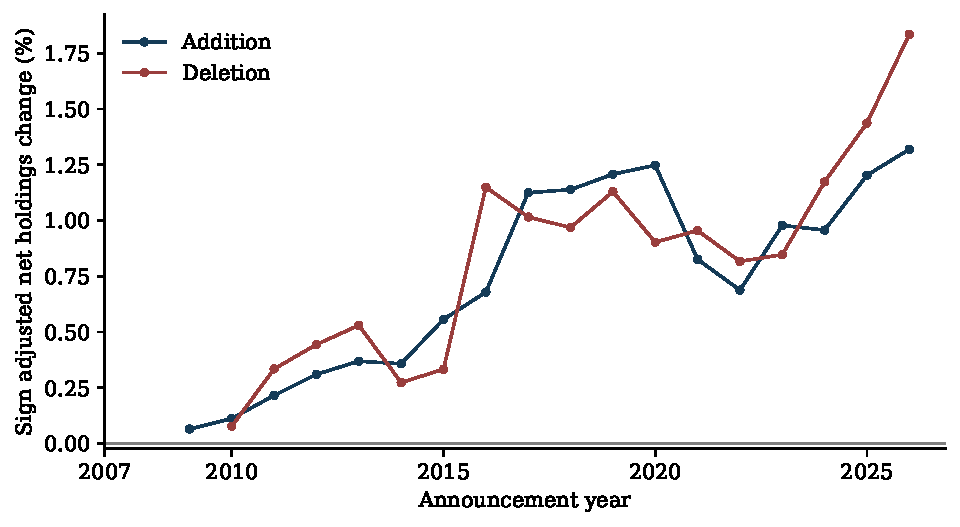
\includegraphics[width=.92\linewidth]{figures/fund_demand.pdf}
\caption{Observed benchmark-linked ownership changes. Annual event means of sign-adjusted net holdings changes as a percentage of shares outstanding. Positive deletion values denote sales. The broad fund definition includes benchmark variants and benchmark-linked mixed-fund holdings. Coverage changes over time; the series is not an estimate of total passive assets or implementation-day orders. The last year is incomplete.}\label{fig:demand}
\end{figure}

The separate FI reporting channel is informative on a matched recent sample. For 106 additions in 2019--2026, measured demand is 1.14\% using FI and 1.05\% using the matched Lipper-based measure. Both use the same mean CAR, 2.43\%, giving ratios of 2.12 and 2.30. This agreement supports the scale of measured later purchases on the overlap. It does not fill missing early reports or establish that either channel captures every relevant investor.

A fixed fund-universe check further separates some coverage change from changes in event composition. Only three funds satisfy the selected mandate and report-availability requirements at every later-decade review; none do so across the whole 2007--2026 period. Within each block, using the same events for the fixed and broad fund measures, fixed-universe addition demand falls from approximately 0.49\% to 0.38\% between the two later blocks, compared with 1.11\% to 0.97\% in the broad measure. The smaller denominator describes a narrower investor population, not a correction that recovers total demand. Appendix~\ref{app:holdings} gives the definition and results.

The holdings evidence thus supports a measured trading association and a useful recent cross-source comparison. It does not establish a precise long-run elasticity trend. The difference from the anchor's US argument is substantive: here, the historical denominator is too coverage-sensitive to carry a strong claim about how efficiently the market absorbs a fixed amount of demand.

\subsection{Trading concentration and liquidity}

The return results do not mean that portfolio adjustment has become unimportant. The final trading day before effectiveness accounts for 9.44\% of the 45-day volume window for early additions and 15.24\% for latest-period additions. The increase is 5.79 percentage points, with a 95\% interval of [3.30, 8.84]. Deletions show a similar increase, from 8.75\% to 14.52\%, a difference of 5.76 points with an interval of [3.26, 8.38].

\begin{figure}[!htbp]\centering
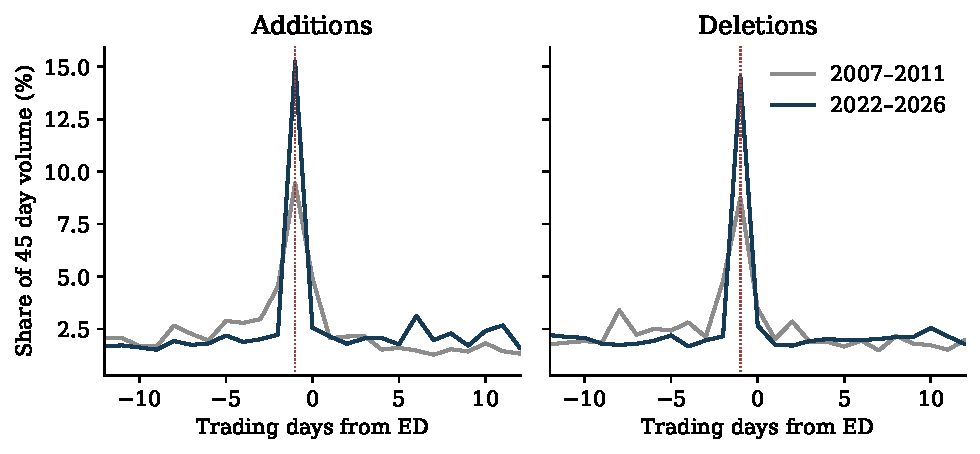
\includegraphics[width=.96\linewidth]{figures/volume_concentration.pdf}
\caption{Trading concentrates immediately before effectiveness. Daily volume as a percentage of each event's total over ED-22 through ED+22; the graph displays ED-12 through ED+12. The dotted line marks ED-1, the final trading day before the new portfolio takes effect. Missing volume is set to zero in this measure. Daily observations do not separate auction and continuous trading.}\label{fig:volume}
\end{figure}

More concentrated trading can coexist with a small implementation-window return. The latest addition implementation CAR is -0.09\%, whereas the announcement CAR is 1.20\%. Investors may anticipate demand or supply liquidity when funds rebalance; prices may also respond to information at other points in the interval. The daily data do not identify which explanation dominates. What they do establish is that the distribution of measured trading around implementation changes even when the mean return near implementation is small.

The spread series supplies context. The value-weighted closing quoted spread among OMXSB members falls from 0.270\% in 2007 to 0.079\% in 2025; the partial 2026 value is 0.087\%. This is consistent with lower quoted trading frictions. It is a different object from the effective spreads and implementation costs examined in the US paper. A closing quote does not measure market depth or the price impact of a large predictable order, so the spread decline cannot establish that improved liquidity caused the return pattern. The annual series is retained in Appendix~\ref{app:additional}.

\FloatBarrier
